\documentclass{article}
\usepackage[a4paper, left=1in, right=1in, top=1in, bottom=1in]{geometry}
\usepackage{amsmath}
\usepackage{graphicx}
\usepackage{xcolor}


\title{Experiment 3: Position Control Using a DC Motor}
\date{}

\begin{document}
\maketitle

\section{Objective}
The objective of this laboratory project is to develop an understanding of Proportional and Derivative (PD) Control as applied to a position control application. In particular, you will explore:
\begin{itemize}
    \item Qualitative properties of proportional and derivative action.
    \item Design of controllers for specifications on the set-point response.
    \item Tracking of triangular signals.
\end{itemize}

\section{Introduction}
The following nomenclature, as described in Table 3.1, is used.

\begin{table}[h]
    \centering
    \begin{tabular}{|c|c|c|}
        \hline
        \textbf{Symbol} & \textbf{Description} & \textbf{Units} \\
        \hline
        $\theta_m$ & Motor angle & rad \\
        $\omega_m$ & Motor angular velocity & rad/s \\
        $u_m$ & Voltage from amplifier which drives the motor & V \\
        $u_e$ & Back-emf voltage & V \\
        $T_m$ & Torque generated by motor & Nm \\
        $T_d$ & Disturbance torque externally applied to the inertial load & Nm \\
        $V_d$ & Disturbance voltage corresponding to $T_d$ & V \\
        $V_{sd}$ & Simulated disturbance voltage & V \\
        $i_m$ & Motor armature current & A \\
        $k_m$ & Motor torque constant & Nm/A \\
        $R_m$ & Motor armature resistance & $\Omega$ \\
        $J_{eq}$ & Total moment of inertia of motor rotor and the load & kg$m^2$ \\
        $K$ & Open-loop steady-state gain & rad/(V.s) \\
        $\tau$ & Open-loop time constant & s \\
        $\omega_n$ & Undamped Natural Frequency & rad \\
        $\zeta$ & Damping Ratio & - \\
        $k_p$ & Proportional gain & V.s/rad \\
        $k_d$ & Derivative gain & V/rad \\
        $b_{sp}$ & Set-Point Weight on proportional Control & - \\
        $b_{sd}$ & Set-Point weight on derivative Control & - \\
        $u$ & Control signal & V \\
        $r$ & Reference signal & rad/s \\
        $y$ & Measured process output & rad/s \\
        \hline
    \end{tabular}
    \caption{Nomenclature used for position control}
\end{table}

Consider a DC motor whose angular position $\theta_m(t)$ is supposed to follow a reference signal $r(t)$. Such a system can be represented by the block diagram shown in Figure 3.1. This block diagram illustrates the parts of the system that are relevant for position control:

\begin{figure}[h]
    \centering
    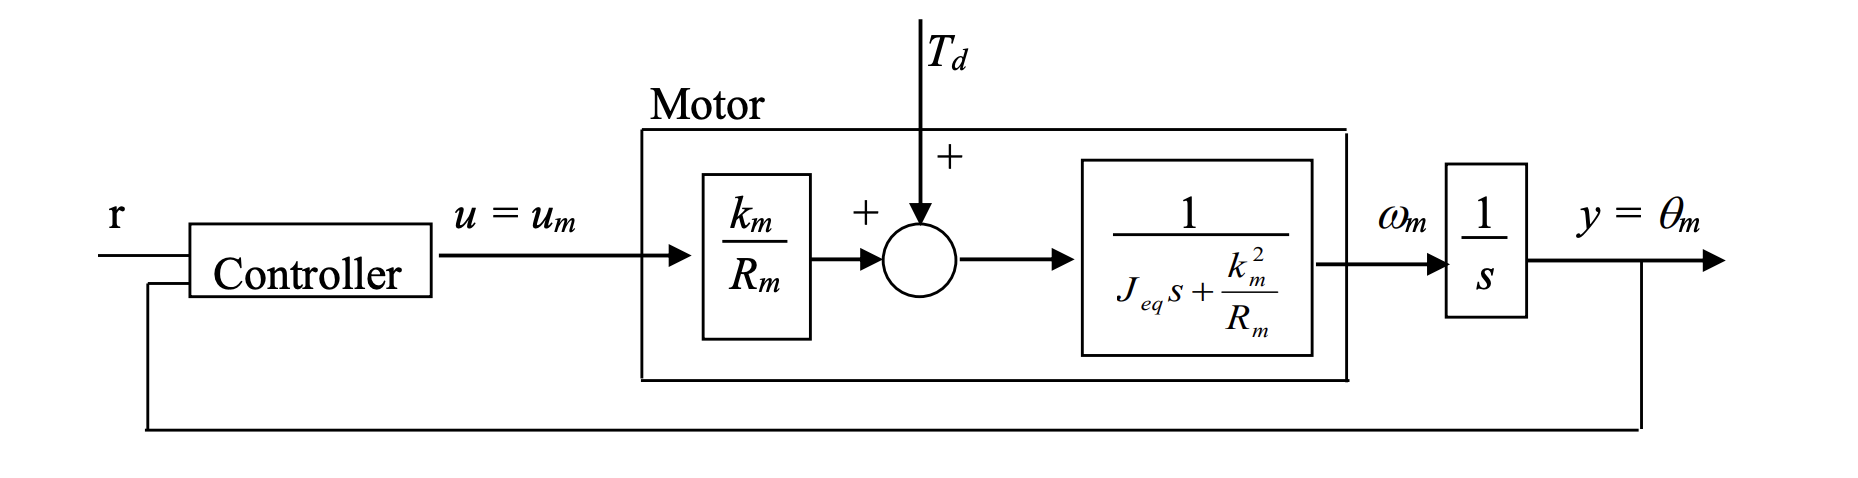
\includegraphics[width=0.7\textwidth]{./block_diagram.png}
    \caption{Block diagram of a position control system}
\end{figure}

The process is represented by a block which has input voltage $u_m$ and torque $T_d$ as inputs and motor angle $\theta_m$ as the output. The torque is typically a disturbance torque similar to the disturbance torque used in experiment 2. The controller to be used in this experiment will be proportional and derivative (PD) control.

\section*{2.1\ \ PD Control Law}
The controller function in Fig. 3.1 can be described using the following equation:
\begin{equation}
    u_m(t) = k_p \left( b_{sp} r(t) - \theta_m(t) \right) + k_d \left[ b_{sd} \frac{\partial}{\partial t} r(t) - \frac{\partial}{\partial t} \theta_m(t) \right]
\end{equation}
where
\begin{itemize}
    \item $k_p$: Proportional Gain
    \item $k_d$: Derivative Gain
    \item $b_{sp}$: Reference Signal Weight for Proportional Part
    \item $b_{sd}$: Reference Signal Weight for Derivative Part
\end{itemize}

The derivative term can be seen as a predictor of future measurements and improves the possibility of introducing damping. One possible disadvantage of derivative control is that it may be noise sensitive due to differentiation.

\section{Pre-Laboratory Assignments}

You may find the short videos discussing the theory behind the preparatory questions useful: \\
\texttt{https://www.youtube.com/watch?v=QX4b-9BcIY4\&list=PLJ-LoEuClIty7ewNzrOhHwqw20VoEXBHBmlz}

\subsection{Proportional Control}
\begin{itemize}
    \item[3.1.1.] The open-loop transfer function between the control input $u_m(t)$ and the position signal $\theta_m(t)$ of the DC motor in Fig. 3.1 can be given by:
    \begin{equation}
        G(s) = \frac{\theta_m(s)}{U_m(s)} = \frac{K}{\tau s + 1} \times \frac{1}{s}
    \end{equation}
    Using the values of $K$ and $\tau$ obtained in experiment 1 and proportional control,
    \begin{equation}
        u_m(t) = k_p (r(t) - \theta_m(t))
    \end{equation}

    \textcolor{blue}{\textbf{Solution:} The open-loop transfer function for the system is:
    \[
    G(s) = \frac{K}{(\tau s + 1) s}
    \]
    Using proportional control, the closed-loop transfer function is given by:
    \[
    \frac{\theta_m(s)}{R(s)} = \frac{k_p K}{s(\tau s + 1) + k_p K}
    \]}

    \item[3.1.2.] Determine the location of the poles of the closed-loop system when the proportional gain $k_p$ is changed. That is, derive the poles of the closed-loop system as a function of $k_p$. How does the unit step response of the system change when $k_p$ is changed?

    \textcolor{blue}{\textbf{Solution:} The characteristic equation of the closed-loop system is:
    \[
    \tau s^2 + s + k_p K = 0
    \]
    The poles are given by:
    \[
    s = \frac{-1 \pm \sqrt{1 - 4\tau k_p K}}{2\tau}
    \]
    As $k_p$ increases, the poles move left, leading to faster responses and reduced settling time. For large $k_p$, the system may become underdamped, resulting in oscillations. For small $k_p$, the system remains overdamped with slower responses.}

    \item[3.1.3.] Consider a step of amplitude $r_0$ for $r(t)$ and use the Final Value Theorem to find $\theta_{ss}$, the value of the output signal of the closed-loop system at steady state. How does it compare to the input signal $r(t)$?

    \textcolor{blue}{\textbf{Solution:} Using the Final Value Theorem:
    \[
    \theta_{ss} = \lim_{s \to 0} s \cdot \frac{k_p K}{s(\tau s + 1) + k_p K} \cdot \frac{r_0}{s}
    \]
    Simplifying:
    \[
    \theta_{ss} = r_0
    \]
    Therefore, with proportional control, the steady-state output equals the reference input, meaning there is no steady-state error for step inputs.}
\end{itemize}

\subsection{Design of Proportional and Derivative Control Parameters}
\begin{itemize}
    \item[3.2.1.] Using the open-loop transfer function, eq. (2) and PD control, eq. (1) with $b_{sp}=1$, obtain the closed-loop transfer function $G_{PD}(s)$ between the reference signal $r(t)$ as input and the motor position $\theta_m(t)$ as output (Assume disturbance torque $T_d = 0$).
    
    \textcolor{blue}{\textbf{Solution:} The open-loop transfer function is:
    \[
    G(s) = \frac{K}{(\tau s + 1) s}
    \]
    Using PD control with $b_{sp}=1$ and $T_d=0$, the control law is:
    \[
    u_m(t) = k_p (r(t) - \theta_m(t)) + k_d \left( \dot{r}(t) - \dot{\theta}_m(t) \right)
    \]
    In Laplace domain:
    \[
    U_m(s) = k_p (R(s) - \Theta_m(s)) + k_d s (R(s) - \Theta_m(s))
    \]
    The closed-loop transfer function $G_{PD}(s)$ is:
    \[
    G_{PD}(s) = \frac{\theta_m(s)}{r(s)} = \frac{K(k_p + k_d s)}{s(\tau s + 1) + K(k_p + k_d s)}
    \]}

    \item[3.2.2.] One possible way to design a controller is to choose controller parameters that give a specified transfer function. The controller parameters can be determined by using the mathematical model of the process and applying pole placement design. Determine the PD controller parameters $k_p$, $k_d$, and $b_{sd}$ so that the closed-loop system, i.e., $G_{PD}(s)$, becomes the following quadratic transfer function:
    \begin{equation}
        G(s) = \frac{\omega_n^2}{s^2 + 2\zeta \omega_n s + \omega_n^2}
    \end{equation}

    \textcolor{blue}{\textbf{Solution:} Comparing coefficients:
    \[
    \tau s^2 + (1 + K k_d)s + K k_p = s^2 + 2\zeta \omega_n s + \omega_n^2
    \]
    Therefore:
    \[
    k_d = \frac{2\zeta \omega_n \tau - 1}{K}, \quad k_p = \frac{\omega_n^2 \tau}{K}, \quad b_{sd} = 1
    \]}

    \item[3.2.3.] For a second order system, eq. (4), with two complex conjugate poles (underdamped), the maximum Percentage Overshoot, $PO$, over the steady-state response is given by:
    \begin{equation}
        PO = 100 e^{\left(\frac{-\pi \zeta}{\sqrt{1-\zeta^2}}\right)}
    \end{equation}
    
    The time to first peak $t_p$ is given by:
    \begin{equation}
        t_p = \frac{\pi}{\omega_n \sqrt{1-\zeta^2}}
    \end{equation}
    
    and the settling time is given by:
    \begin{equation}
        T_s = \frac{4}{\zeta \omega_n}
    \end{equation}
    
    Using the following values as design specifications:
    \begin{equation}
        PO \leq 18\% \quad \text{and} \quad T_s = 0.43 \, s
    \end{equation}
    
    choose a damping ratio, $\zeta$, and a natural frequency $\omega_n$, that satisfies the above requirements. Is the value $\zeta = 0.5$ acceptable? Explain.
    
    \textcolor{blue}{\textbf{Solution:} First, for $PO \leq 18\%$, we use the overshoot formula:
    \[
    PO = 100 e^{\left(\frac{-\pi \zeta}{\sqrt{1-\zeta^2}}\right)} \leq 18
    \]
    Solving this inequality gives $\zeta \geq 0.48$. Now, using the settling time formula $T_s = \frac{4}{\zeta \omega_n}$, and substituting $T_s = 0.43$ s, we get:
    \[
    0.43 = \frac{4}{\zeta \omega_n}
    \]
    Choosing $\zeta = 0.5$, we find:
    \[
    \omega_n = \frac{4}{0.43 \times 0.5} \approx 18.6 \, \text{rad/s}
    \]
    Hence, $\zeta = 0.5$ is acceptable as it satisfies both the overshoot and settling time requirements.}

    \item[3.2.4.] Using the numerical results from 3.2.3 and the expressions derived for $k_p$, $k_d$, and $b_{sd}$ in 3.2.2 compute $k_p$, $k_d$, and $b_{sd}$.

    \textcolor{blue}{\textbf{Solution:} Using the values $\zeta = 0.5$ and $\omega_n = 18.6$ rad/s from 3.2.3, we substitute them into the formulas for $k_p$ and $k_d$ derived in 3.2.2:
    \[
    k_p = \frac{(18.6)^2 \cdot \tau}{K}, \quad k_d = \frac{2(0.5)(18.6) - 1}{K}, \quad b_{sd} = 1
    \]
    The exact values of $k_p$ and $k_d$ depend on the values of $\tau$ and $K$ obtained in experiment 1.}

    \item[3.2.5.] Consider a step with amplitude $r_0$ for $r(t)$ and use the Final Value Theorem to find $\theta_{ss\_ PD}$, the value of the output signal $\theta_m$ of the closed-loop system at steady state. How does it compare to the input signal $r(t)$?

    \textcolor{blue}{\textbf{Solution:} Using the Final Value Theorem:
    \[
    \theta_{ss\_ PD} = \lim_{s \to 0} s \cdot \Theta_m(s)
    \]
    The transfer function is:
    \[
    \Theta_m(s) = \frac{\omega_n^2}{s^2 + 2\zeta \omega_n s + \omega_n^2} \cdot \frac{r_0}{s}
    \]
    Simplifying for $s \to 0$, we find that:
    \[
    \theta_{ss\_ PD} = r_0
    \]
    This shows that with PD control, there is no steady-state error, and the output tracks the reference signal exactly.}
\end{itemize}


\subsection{Tracking Triangular Signals}
\begin{itemize}
    \item[3.3.1.] Consider the closed-loop system with PD control, i.e., $G_{PD}(s)$, and assume that you have as input a ramp signal given by:
    \begin{equation}
        r(t) = r_0 \, t \quad \text{for} \quad t \geq 0
    \end{equation}
    
    Apply the Final Value Theorem to calculate the steady-state error, $e_{ss\_ PD}$.

    \textcolor{blue}{\textbf{Solution:} For a ramp input $r(t) = r_0 t$, with Laplace transform $R(s) = \frac{r_0}{s^2}$:
    \[
    e_{ss\_ PD} = \lim_{s \to 0} s \cdot \frac{s R(s)}{1 + G_{PD}(s)}
    \]
    Using the designed quadratic transfer function:
    \[
    e_{ss\_ PD} = \frac{r_0}{\omega_n^2}
    \]}

    \item[3.3.2.] Compute $e_{ss\_ PD}$ using $r_0 = 32$ [rad/s] and the values of $k_p$, $k_d$, and $b_{sd}$ obtained in 3.2.4.
    
    \textcolor{blue}{\textbf{Solution:} Using $r_0 = 32$ rad/s and $\omega_n = 18.6$ rad/s:
    \[
    e_{ss\_ PD} = \frac{32}{(18.6)^2} \approx 0.09 \text{ rad}
    \]}
\end{itemize}

\subsection{Pre-Laboratory Results Summary Table}

\begin{table}[h!]
    \centering
    \begin{tabular}{|l|c|c|c|}
    \hline
    \textbf{Description} & \textbf{Symbol} & \textbf{Value} & \textbf{Units} \\ \hline
    Open-loop steady-state gain & $K$ & \textcolor{blue}{19.92} & rad/(V.s) \\ \hline
    Open-loop time constant & $\tau$ & \textcolor{blue}{0.093} & s \\ \hline
    \multicolumn{4}{|c|}{\textbf{PD Controller Design}} \\ \hline
    Proportional Gain & $k_p$ & \textcolor{blue}{32.15} & V/rad \\ \hline
    Derivative Gain & $k_d$ & \textcolor{blue}{0.93} & V.s/rad \\ \hline
    Set-Point Weight on Derivative Part & $b_{sd}$ & \textcolor{blue}{1} &  \\ \hline
    Desired Damping Ratio & $\zeta$ & \textcolor{blue}{0.5} &  \\ \hline
    Desired Undamped Natural Frequency & $\omega_n$ & \textcolor{blue}{18.6} & rad/s \\ \hline
    Given Maximum Percentage Overshoot & $PO$ & \textcolor{blue}{$\leq 18$} & \% \\ \hline
    Given 2\% Settling Time & $T_s$ & \textcolor{blue}{0.43} & s \\ \hline
    Desired Peak Time & $t_p$ & \textcolor{blue}{0.19} & s \\ \hline
    Steady-State Value of Position using PD & $\theta_{ss\_ PD}$ & \textcolor{blue}{32} & rad \\ \hline
    \multicolumn{4}{|c|}{\textbf{Tracking Triangular Signals}} \\ \hline
    Steady-State Error using PD control & $e_{ss\_ PD}$ & \textcolor{blue}{0.09} & rad \\ \hline
    \end{tabular}
    \caption{Position Control pre-laboratory assignment results}
\end{table}

\section{In-Laboratory Session}
\subsection{Position Control Module}
The \textit{Position Control} module of the QICii software package is the main tool for this laboratory.
\begin{figure}[h!]
    \centering
    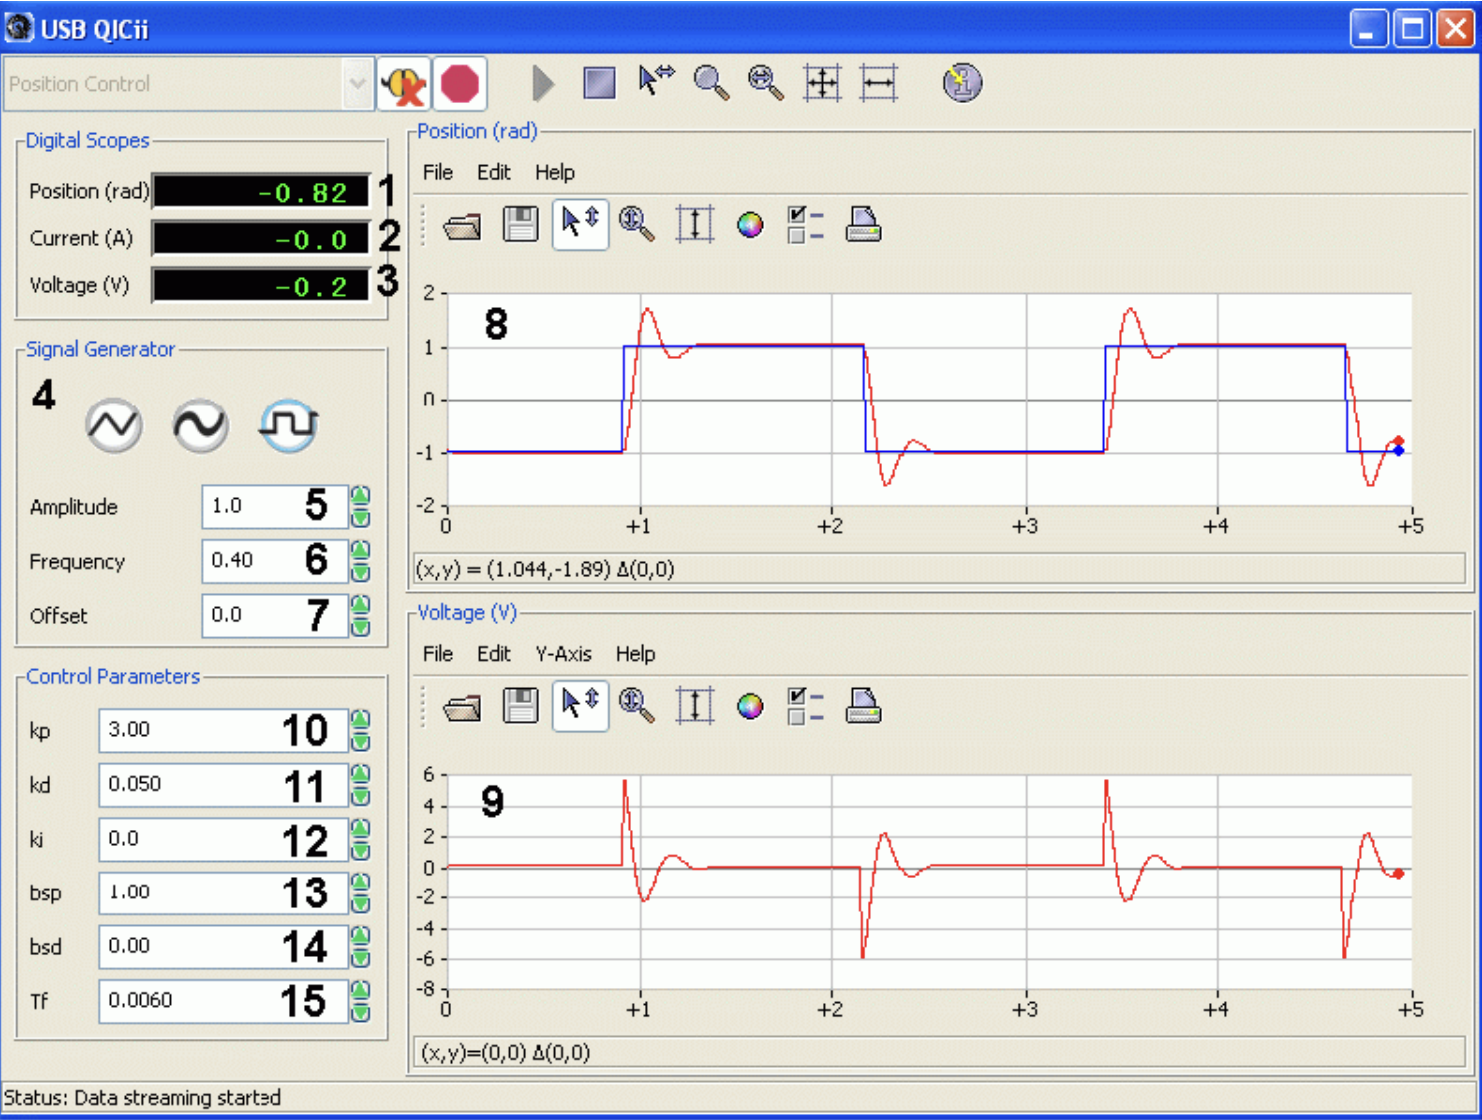
\includegraphics[width=0.9\textwidth]{./USBQICii.png}
    \caption{Interface of the Position Control module.}
\end{figure}

\begin{table}[h!]
    \centering
    \begin{tabular}{|c|l|c|p{5.5cm}|c|}
    \hline
    \textbf{ID \#} & \textbf{Label} & \textbf{Parameter} & \textbf{Description} & \textbf{Unit} \\ \hline
    1  & Position    & $\theta_m$  & Motor Output position Numeric Display     & rad   \\ \hline
    2  & Current     & $i_m$       & Motor Armature Current Numeric Display    & A     \\ \hline
    3  & Voltage     & $u_m$       & Motor Input Voltage Numeric Display       & V     \\ \hline
    4  & Signal Generator & & Type of Generator for the Angle Reference Signal: Sawtooth Wave or Square Wave & \\ \hline
    5  & Amplitude   &             & Generated Signal Amplitude Input Box      & rad   \\ \hline
    6  & Frequency   &             & Generated Signal Frequency Input Box      & Hz    \\ \hline
    7  & Offset      &             & Generated Signal Offset Input Box         & rad   \\ \hline
    8  & Speed       & $\omega_m$  & Scope with Actual (in red) and Reference (in blue) Angles & rad \\ \hline
    9  & Voltage     & $u_m$       & Scope with Applied Motor Voltage (in red) & V     \\ \hline
    10 & kp          & $k_p$       & Controller Proportional Gain Input Box     & V/rad \\ \hline
    11 & kd          & $k_d$       & Controller Derivative Gain Input Box       & V.s/rad \\ \hline
    12 & ki          & $k_i$       & Controller Integral Gain Input Box         & V/(rad.s) \\ \hline
    13 & bsp         & $b_{sp}$    & Controller Proportional Reference Signal Weight Input Box & \\ \hline
    14 & bsd         & $b_{sd}$    & Controller Derivative Reference Signal Weight Input Box   & \\ \hline
    15 & Tf          & $T_f$       & Time Constant of Filter for obtaining the Derivative of the Error Signal & s \\ \hline
    \end{tabular}
    \caption{QICii Position Control Module Nomenclature}
\end{table}

\textbf{Table 3.3.} Lists and describes the main elements of the \textit{Position Control} module interface.\\\\\\\\\\

The \textit{Position Control} module program runs the process in closed-loop with the motor reference position angle given by the signal generator. There are two windows that show the time histories of motor position (control output) and motor voltage (control input).
To compute the control signal, eq. (1), it is required that the term:
\[
e_d(t) = \frac{\partial}{\partial t} \left( b_{sd}r(t) - \theta_m(t) \right)
\tag{10}
\]
is computed. The signal \( e_d(t) \) is obtained by filtering the error signal using the following filter:
\[
E_d(s) = \frac{s}{T_f s + 1} \left[ b_{sp}R(s) - \Theta_m(s) \right]
\tag{11}
\]
where \( E_d(s) \), \( R(s) \), and \( \Theta_m(s) \) are the Laplace transforms of the signals \( e_d(t) \), \( r(t) \), and the position \( \theta_m(t) \). A good value for \( T_f \) is 0.006 and should be left unchanged during this experiment.

\section{Quantitative Properties of Proportional and Derivative Control}

The goal of the following procedures is to develop an intuitive feel for the properties of proportional and derivative control actions.

\subsection{Proportional Control}

\textbf{Step 1.} Set reference signal to a square wave. A reasonable amplitude is 3 rad. When you change the reference signal level ensure that the control signal does not saturate. Set both integral and derivative gains to zero (\(k_i = k_d = 0\)). Set the proportional gain to 0.2 V/rad to start with. Ensure that the following parameters of the Position Control window are set properly.
\[
\begin{array}{|c|c|c|c|c|c|}
\hline
\text{Signal Type} & \text{Amplitude [rad]} & \text{Frequency [Hz]} & \text{Offset [rad]} & k_p \, [V/\text{rad}] & b_{sp} \\
\hline
\text{Square Wave} & 3 & 0.4 & 0 & 0.2 & 1 \\
\hline
\end{array}
\]
\textbf{Step 2.} To investigate the closed-loop system for proportional controllers with different gains change the proportional gain to the following values: \( k_p = 1 \), \( 2 \), and \( 4 \, V/\text{rad} \). What are your observations?

\textbf{Step 3.} Describe the steady-state error to a step input.

\textbf{Step 4.} Repeat the previous observations. Change the Amplitude of the reference signal and observe under what conditions the control signal saturates.
\section{Proportional and Derivative (PD) Control}

The combination of proportional and derivative control will now be explored. Follow the steps below:

\textbf{Step 1.} Fix the proportional gain to 2.0 V/rad and set the derivative gain to 0.0 V.s/rad to start with (\(b_{sp} = b_{sd} = 1\)). Set the parameters of the QICii module window as listed in Table 3.5. Set the integral gain to zero (\(k_i = 0\)).

\[
\begin{array}{|c|c|c|c|c|c|c|c|}
\hline
\text{Signal Type} & \text{Amplitude [rad]} & \text{Frequency [Hz]} & \text{Offset [rad]} & k_p \, [V/\text{rad}] & k_d \, [V\cdot s/\text{rad}] & b_{sp} & b_{sd} \\
\hline
\text{Square Wave} & 2 & 0.4 & 0 & 2.0 & 0 & 1 & 1 \\
\hline
\end{array}
\]
\begin{center}
\text{Table 3.5. Module Parameters for the Proportional and Derivative Control Test}
\end{center}

\textbf{Step 2.} Change the derivative gain by incremental steps of 0.05 V.s/rad to investigate the closed-loop system for PD controllers with different derivative gains. Try the following gains: \( k_d = 0 \), 0.05, 0.1, and 0.15 V.s/rad. What are your observations?

\textbf{Step 3.} Determine the lowest value of derivative gain \( k_d \) which gives a step response without overshoot (\(k_p\) still 2 V/rad). Determine the settling time for the closed loop system.

\section{PD Controller Design to Given Specifications}

This section provides the experimental verification of the PD controller design to given specifications, as carried out in the pre-lab assignment in Section 3.2. The performance of the closed-loop system with the control parameters obtained using the basic pole assignment method in Section 3.2. will be evaluated and compared to the performance specifications given in eq. (8). Please follow the steps below:

\textbf{Step 1.} Set the parameters of the QICii module window as described in Table 3.6.

\[
\begin{array}{|c|c|c|c|c|c|}
\hline
\text{Signal Type} & \text{Frequency [Hz]} & \text{Amplitude [rad]} & \text{Offset [rad]} & b_{sp} & T_f \, [s] \\
\hline
\text{Square Wave} & 0.4 & 4.5 & 0 & 1 & 0.006 \\
\hline
\end{array}
\]
\begin{center}
\text{Table 3.6. Module Parameters for PD Controller Design to Given Specifications}
\end{center}

Ensure that the integral gain is zero (\(k_i = 0\)) and set \(b_{sd}\) and both proportional and derivative gains, \(k_p\) and \(k_d\), to the values you calculated in Section 3.2, Question 3.2.4.

\textbf{Step 2.} Make sure that the motor input voltage is below its saturation limit. If not, adjust the square wave reference signal Amplitude. Measure the resulting Percent Overshoot (PO), settling time \(T_s\), and peak time \(t_p\). Does the system's actual response meet the desired requirements? How close are the measurements to the values you calculated in Question 3.2.3?

\textbf{Step 3.} Summarize your observations and your calculations in your report. Select some representative results, screen-captures, and plots.

\section{Tracking Triangular Signals}

\textbf{Step 1.} Select a triangular reference signal and set the parameters of the QICii module window as listed in Table 3.7. Set the controller gains to the PD controller parameters (i.e \(k_p\), \(k_d\), \(b_{sd}\)) to the values calculated in Question 3.2.4.

\[
\begin{array}{|c|c|c|c|c|c|}
\hline
\text{Signal Type} & \text{Amplitude [rad]} & \text{Frequency [Hz]} & \text{Offset [rad]} & b_{sp} & T_f \, [s] \\
\hline
\text{Triangular Wave} & 20 & 0.4 & 0 & 1 & 0.006 \\
\hline
\end{array}
\]
\begin{center}
\text{Table 3.7. QICii Module Parameters for Triangular Wave Tracking Test}
\end{center}

\textbf{Step 2.} From the triangular wave specifications given in Table 3.7, calculate the slope \(r_0\) of the ramp signal (see eq. (9)).

\textbf{Step 3.} Observe how well the output signal tracks the triangular signal (in particular in terms of the tracking error). Measure the actual asymptotic tracking error and compare it with the analytic estimate obtained in Question 3.3.2.

\textbf{Step 4.} Change the controller proportional gain \(k_p\) by steps of \(\pm 0.5 \, V/\text{rad}\) and explore its effect on the tracking error. Select some representative results and plots and include in your report.

\section{References}
\begin{enumerate}
    \item K. Ogata, Modern Control Engineering, 5\textsuperscript{th} Edition, Prentice Hall, Englewood Cliffs, N.J., 2010.
    \item K. J. Astrom, J. Apkarian, H. Lacharery, USB QICii Laboratory Workbook, Quanser Engineering Trainer Series.
\end{enumerate}

\end{document}
